% Chapter 1

\chapter{Interpolated Discretized object pairs embedding} % Main chapter title

\label{Chapter3} % For referencing the chapter elsewhere, use \ref{Chapter1} 

We now describe the Interpolated Discretized Distances (IDD) embedding method.
As mentioned above, this method uniqueness is applying an embedding method that treats each pair as a \textbf{joint} object in its problem.
This method may fit any two-objects task such similarity/matching problems etc. 
Let us initiate by presenting the original single dimensional (IDD-1D) work[], then the expansion of this work into multidimensional (IDD-ND) scenario - general distance embedding is described.

\section{1D case}

	Our method's objective is to find an embedding function such:
	
	\begin{equation}
		ID:\Re^n \times \Re^m \rightarrow \Re^d
	\end{equation}
	, which applies the following distance function by multiplying with a learned weights vector $\overrightarrow{w}$ (learned vector)
	
	\begin{equation}
	d(\overrightarrow{x_1} , \overrightarrow{x_2}) = ID(\overrightarrow{x_1} , \overrightarrow{x_2}) \times \overrightarrow{w}
	\end{equation}
	
	this embedding shall obtain semimetric constraints applied.
	
	\subsection{Discretization}

	\begin{figure}
		
		\qquad \qquad \qquad \quad \begin{pmatrix} c_{1(1)} , \dots , \dots , \dots , c_{1(n)} \end{pmatrix}\\
		
		$W$ =		\begin{pmatrix} c_{2(1)} \\ \vdots \\ \vdots \\ \vdots \\ \vdots \\c_{2(m)} \end{pmatrix}
		\begin{pmatrix}
			s_{1,1}&   \dots&   \dots&   \dots& s_{1,m}\\
			\vdots& \ddots &        &        & \vdots \\
			\vdots&        & \ddots &        & \vdots  \\
			\vdots&        &        & \ddots & \vdots  \\
			\vdots&        &        &        & \vdots  \\
			s_{n,1}  & \dots  & \dots  & \dots  & s_{n,m}
		\end{pmatrix}
		\caption[discretization matrix]
		{discretization matrix $W$ as built from 2 vectors $c_1 , c_2$. this matrix is 2D as it is an outcome of 2 - 1D vectors discretization processes}
	\end{figure}

	
	as described in \ref{Chapter2} 1D-IDD describes bin-to-bin distance between two samples from single dimensional spaces. Each dimension is clustered and sorted into $C_i$ - dimensional: $\overrightarrow{c} \in \Re^{C_i}$ vector.
	The vector's pair defines the shape of a distance matrix $W \in \Re^{C_i \times C_j}$ , where each element $W_i,j$ describes the distance between two cluster centers form vectors - $v_a , v_b$ \\
	
	
	
	\subsection{Interpolation}
	
	As described above , our $IDD$ function provides continuous output for any given valid object/pair of objects. 
	For this purpose we perform interpolation of the given data sample features within the $W$ matrix space for each data sample by the following process:
	\begin{itemize}
		\item extract the closest vertices from $W$ matrix to the feature sample. 
		\item calculate four (2 per feature) coefficients per sample, each represented by the normalized surface of the opposite triangle to a vertex (1D coefficients calculation will be described in section). 
		\item 1D-IDD is computed by applying inner product between the sparse coefficient vector and their corresponding vertices vector:\\
		\begin{equation}
		1DIDD = \sum_{t=1}^{3}\alpha_{a(t),b(t)} \times W_{a(t),b(t)}
		\end{equation}
		where:\\
		$\alpha$ is the coefficients sparse vector , representing the interpolation result per feature vector
		$a , b$ are parametrization function for both $\alpha , W$
		$t$ is the scanning index for all arguments among this expression
	\end{itemize}
		
	Please notice that there are only 4 elements different than zero at $\alpha$, so this expression represents the non-zero elements only provides value to $1DIDD$ expression \\
	
	$a,b$ parameterizations are described as:
	
	\begin{itemize} \label{hypercubes}
		\item	\begin{equation} a_{(1)}=a{(2)} =argmax_{(c_i)} \{ v_{c_i} \leq x_i \} \end{equation}
		\item 	\begin{equation} a_{(3)}=a{(4)} =argmin_{(c_i)} \{ v_{c_i} \geq x_i \}  \end{equation} 
		\item 	\begin{equation} b_{(1)}= b_{(3)} =argmax_{(c_j)} \{ v_{c_j} \leq x_j \}  \end{equation}
		\item 	\begin{equation} b_{(2)}=b_{(4)} =argmin_{(c_j)} \{ v_{c_j} \geq x_j \} \end{equation} 
	\end{itemize}		
	
	\subsubsection{Interpolation Coefficients extraction - 1D}
	
	Let us describe how does coefficients vectors are calculated from a data sample (assembled from a pair of samples) and a discretization matrix.
		
		
	\newcommand{\MyNewVariable}{(0.3 , 0.8)}

				
	\begin{figure}[h]


		\label{fig:32}  
			\centering
			\scalebox{0.6}
			{
				\begin{tikzpicture}[scale=5]
				\tikzstyle{vertex}=[circle,minimum size=20pt,inner sep=0pt]
				\tikzstyle{selected vertex} = [vertex, fill=red!6]
				\tikzstyle{selected edge} = [draw,line width=5pt,-,blue!50]
				\tikzstyle{edge} = [draw,thick,-,black]

				
				%\node[vertex] (v00) at (-3,-3) {$(-3,-3)$};
				\node[vertex] (v01) at (-3,-2) {$(-3,-2)$};
				\node[vertex] (v02) at (-3,-1) {$(-3,-1)$};
				\node[vertex] (v03) at (-3,0) {$(-3,0)$};
				\node[vertex] (v04) at (-3,1) {$(-3,1)$};
				\node[vertex] (v05) at (-3,2) {$(-3,2)$};
				\node[vertex] (v06) at (-3,3) {$(-3,3)$};
				%\node[vertex] (v10) at (-2,-3) {$(-2,-3)$};
				\node[vertex] (v11) at (-2,-2) {$(-2,-2)$};
				\node[vertex] (v12) at (-2,-1) {$(-2,-1)$};
				\node[vertex] (v13) at (-2,0) {$(-2,0)$};
				\node[vertex] (v14) at (-2,1) {$(-2,1)$};
				\node[vertex] (v15) at (-2,2) {$(-2,2)$};
				\node[vertex] (v16) at (-2,3) {$(-2,3)$};
				%\node[vertex] (v20) at (-1,-3) {$(-1,-3)$};
				\node[vertex] (v21) at (-1,-2) {$(-1,-2)$};
				\node[vertex] (v22) at (-1,-1) {$(-1,-1)$};
				\node[vertex] (v23) at (-1,0) {$(-1,0)$};
				\node[vertex] (v24) at (-1,1) {$(-1,1)$};
				\node[vertex] (v25) at (-1,2) {$(-1,2)$};
				\node[vertex] (v26) at (-1,3) {$(-1,3)$};
				%\node[vertex] (v30) at (0,-3) {$(0,-3)$};
				\node[vertex] (v31) at (0,-2) {$(0,-2)$};
				\node[vertex] (v32) at (0,-1) {$(0,-1)$};
				\node[vertex] (v33) at (0,0) {\textcolor{green}{$(0,0)$}};
				\node[vertex] (v34) at (0,1) {\textcolor{red}{$(0,1)$}};
				\node[vertex] (v35) at (0,2) {$(0,2)$};
				\node[vertex] (v36) at (0,3) {$(0,3)$};
				%\node[vertex] (v40) at (1,-3) {$(1,-3)$};
				\node[vertex] (v41) at (1,-2) {$(1,-2)$};
				\node[vertex] (v42) at (1,-1) {$(1,-1)$};
				\node[vertex] (v43) at (1,0) {$(1,0)$};
				\node[vertex] (v44) at (1,1) {\textcolor{blue}{$(1,1)$}};
				\node[vertex] (v45) at (1,2) {$(1,2)$};
				\node[vertex] (v46) at (1,3) {$(1,3)$};
				%\node[vertex] (v50) at (2,-3) {$(2,-3)$};
				\node[vertex] (v51) at (2,-2) {$(2,-2)$};
				\node[vertex] (v52) at (2,-1) {$(2,-1)$};
				\node[vertex] (v53) at (2,0) {$(2,0)$};
				\node[vertex] (v54) at (2,1) {$(2,1)$};
				\node[vertex] (v55) at (2,2) {$(2,2)$};
				\node[vertex] (v56) at (2,3) {$(2,3)$};
				\node[vertex] (v60) at \MyNewVariable {};
			
				%\draw[edge] (v00) -- (v01) -- (v02) -- (v03) -- (v04) -- (v05) -- (v06);
				\draw[edge] (v01) -- (v02) -- (v03) -- (v04) -- (v05) -- (v06);
				\draw[edge] (v11) -- (v12) -- (v13) -- (v14) -- (v15) -- (v16);
				\draw[edge] (v21) -- (v22) -- (v23) -- (v24) -- (v25) -- (v26);
				\draw[edge] (v31) -- (v32) -- (v33) -- (v34) -- (v35) -- (v36);
				\draw[edge] (v41) -- (v42) -- (v43) -- (v44) -- (v45) -- (v46);
				\draw[edge] (v51) -- (v52) -- (v53) -- (v54) -- (v55) -- (v56);
				%\draw[edge] (v00) -- (v10) -- (v20) -- (v30) -- (v40) -- (v50);
				\draw[edge] (v01) -- (v11) -- (v21) -- (v31) -- (v41) -- (v51);
				\draw[edge] (v02) -- (v12) -- (v22) -- (v32) -- (v42) -- (v52);
				\draw[edge] (v03) -- (v13) -- (v23) -- (v33) -- (v43) -- (v53);
				\draw[edge] (v04) -- (v14) -- (v24) -- (v34) -- (v44) -- (v54);
				\draw[edge] (v05) -- (v15) -- (v25) -- (v35) -- (v45) -- (v55);
				\draw[edge] (v06) -- (v16) -- (v26) -- (v36) -- (v46) -- (v56);
				
				\fill \MyNewVariable circle(1.3pt);
				\draw[edge] (v60) -- (v34);
				\draw[edge] (v60) -- (v44);
				\draw[edge] (v60) -- (v33);
				\draw[edge] (v44) -- (v33);
	
				 \fill[red] (0.01,0.01) -- (0.99,0.99) -- \MyNewVariable -- cycle;
				 \fill[green] (0.01,0.99) -- (0.99,0.99) -- \MyNewVariable -- cycle;
				 \fill[blue] (0.01,0.01) -- (0.01,0.99) -- \MyNewVariable -- cycle;
				\fill \MyNewVariable circle(1.3pt);
				
				
				\end{tikzpicture}}
		\captionsetup{width=1.2\linewidth}		
		\caption[1D data sample coefficients calculation matrix]
		{this matrix scheme describes a given data sample coefficients calculation according to its containing hypercube and simplex.The examined data sample is $(0.3 , 0.8)$, so its containing hypercube would be the cell between $[0,1]$. 
		In this hypercube we search the containing simplex (triangle in 1D case), which occurs to be the upper triangle among the 2 main diagonal triangles. By assembling 3 sub-triangles using the data sample and the vertices we  may extract the proper coefficients for the ID vector. Each normalized sub-triangle surface represents the contrary vertex's coefficients. For example the \textcolor{blue}{blue} triangle surface correlates with the \textcolor{blue}{$(1,1)$} vertex's coefficient , 
		the \textcolor{green}{green} surface correlates with the \textcolor{green}{$(0,0)$} vertex's coefficient and
		the \textcolor{red}{red} surface correlates with the \textcolor{red}{$(0,1)$} vertex's coefficient.}
		

		\end{figure} 
		
		
		
		
		
		
		
		For a given data pair, bounding square (2D-cube) is assembles from the clusters vectors per feature.
		this square is divided into 2 triangles (simplices) along its main diagonal, as described in figure \ref{fig:32}.
		
		The containing triangle of the data sample is divided to 3 sub-triangles by applying direct lines between the data sample and each vertex of the relevant triangle. Each sub-triangle relative surface represents the coefficient of the opposite vertex \ref{fig:32}. \\ 
		In the 1D case, there would be just \textbf{3} non-zero elements in the ID coef. vector, since there are 3 affecting sub-triangles (the forth vertex of the cell is zeroed like any other vertex in the output ID vector) .
				
		Single dimensional formation $IDD$ applies semi-metrics properties as described back in \ref{Chapter1}
		
			
	\subsection{Assigning}
	Now that we have ID coefficients (sparse) vector, we may assign it to the ID output vector shape.
	ID output vector is sized by the flatten vector of the discretization matrix $W$, which may be flatten row-wise/column-wise \ref{flatt}.\\
	Each vertex in the output vector receives the value calculated for its equivalent index at the opposite triangles surfaces phase.
	


\section{multidimensional case}

We now address describing the generalization of the single dimension IDD method to n-dimensional object pairs embedding. \\
For this we should adapt a different embedding attitude, since it should obtain multi-dimensional embedding, unlike the triangles relative surfaces process performed in the 1d scenario.  \\
The selected coefficients calculation process for our embedding is the Barycentric (center of mass) Coordinates [] of a given vector in a 2n dimensional space (2n since we embed pairs of objects for distance/similarity calculation).

	\subsection{Definition}
	
	The general expression of $NDIDD$ would appear to be:
	\begin{equation}
			NDIDD = \sum_{t=1}^{2n!}\alpha_{a(t),b(t)} \times W_{a(t),b(t)}
	\end{equation}
	
	In this scenario, $a , b$ are the multi-dimensional parametrization functions, which correlates between the coefficients vector and the learned weights vector.

		
	\subsection{Discretization}
	Given a n-dimensional vectors dataset, we first discrete the data range/space of each dimension, into $C$ discretization values. 
	$C$ may vary among dimensions. This step is equivalent to the 1D scenario.
	At the 1D scenario, a 2D matrix was generated, which represents the distance between a pair of elements.
	
	Now we address the n-dimensional scenario, by obtaining a $2n$ dimensional tensor, representing the distance between a pair of n dimensional vectors.
	
	\subsection{Interpolation}
	
	Next phase is interpolating every dataset sample, or any tested sample, in order to embed it using our method.
	
	let us assign a pair of n-dimensional vectors $x_1 , x_2 \in \Re^n$.\\
	$NDIDD$ embedding handles this pair as a \textbf{joint 2n dimensional vector}, flatten in the following order:\\
	\begin{equation}
		\overrightarrow{p} = [x_1^1 , x_2^1 , ... , ... , x_1^n , x_2^n] ,\qquad \overrightarrow{p} \in \Re^{2n}
	\end{equation}
	
	for the further process description we will treat $\overrightarrow{p}$ as our data object
	
	
		\subsubsection{find bounding hypercube}
		First, we place the sampled vector $\overrightarrow{p}$ within its bounding 2n-hypercube, same as performed in the single dimensional scenario \ref{hypercubes}.  
			
		\subsubsection{find bounding simplex}
		
		Next stage is discover the simplex (equivalent to triangle in 1d scenario) containing point $\overrightarrow{p}$.
		A 2n-dimensional hypercube is assembled from $(2n)!$ vertices. 
		Assuming the vertices values are normalized to a “unit hypercube” - containing only $0/1$ values in elements, any vertex applies a permutation as follows:
		
		\begin{equation}
		0 \leq p_{t(1)} \leq p_{t(1)} \leq \dots \leq p_{t(2n-1)} \leq p_{t(2n)} \leq 1
		\end{equation}
		
		http://www.mathpages.com/home/kmath664/kmath664.htm
		
		
		where:\\
		$t_{(i)}$ is a permutation function.
		
		so how we select the right simplex (and permutation) for a given point p?
		Each point $\overrightarrow{p}$ obeys a unique permutation. 
		A certain permutation defines the right simplex vertices. 
		For each set of correct vertices that obeys a certain permutation, the extreme vertices, all zeros/all ones values, always included in the right vertices account. 
		
		
		
		\subsubsection{calculate sub-volumes of all simplices involved}
		
		Next phase is calculating the relative volumes (equivalent to 1 dimensional relative surfaces) of all sub simplices. 
		\\Given a simplex assembled from $T = 2n+1$ set of vertices, which bounds a point $\overrightarrow{p}$, we calculate the volumes of T sub-simplices, so every simplex is assembled from $T-1$ vertices plus $\overrightarrow{p}$. 
		\\These normalized volumes represents the coefficients of the missing (or counter in the T space) vertex.
		
		
		
		\subsubsection{Simplex Volume Calculation}
		
		Given $T = 2n+1$ simplices of $N = 2n$ dimension, a general expression for the volume contained between its vertices would be:
		
	
		\begin{equation}
		V_{[r^1,r^2,r^3,\dots,\dots,r^T]} = \frac{1}{(2n)!} \times \begin{vmatrix}
		1 & r_1^1 & r_2^1 & \dots & r_{2n}^1\\ 
		1 & r_1^2 & \ddots & \ddots & r_{2n}^2\\ 
		\vdots & \ddots & \ddots & \ddots & \vdots \\ 
		\vdots & \ddots & \ddots & \ddots & \vdots\\ 
		1 & r_{1}^T &  \dots& \dots & r_{2n}^T
		\end{vmatrix}
		\end{equation}
				
    	We calculate the volume for every vertex in the simplex as follows:
		Given a point $\overrightarrow{p}$ and a set of vertices $r^1,r^2,r^3,...,r^T$ ,  the volume correspond to every vertex $r^i$ is: 
		
		\begin{equation}
			\lambda_i = 	V_{[r^1,r^2,p,\dots,\dots,r^T]} = \frac{1}{(2n)!} \times \begin{vmatrix}
				1 & r_1^1 & r_2^1 & \dots & r_{2n}^1\\ 
				1 & r_1^2 & \ddots & \ddots & r_{2n}^2\\ 
				\vdots &  p_1  & p_2 & \ddots & p_{2n} \\ 
				\vdots & \ddots & \ddots & \ddots & \vdots\\ 
				1 & r_{1}^T &  \dots& \dots & r_{2n}^T
				\end{vmatrix}
		\end{equation}
			
		\subsubsection{Efficient method - calculating Barycentric Coordinates (BCC)}
		
		A more efficient way (time complexity $O(n)$) providing the coefficients to a given point is by using barycentric coordinates of a point $\overrightarrow{p}$.
		Given a point $\overrightarrow{p} \in \Re^{2n}$ , the following formulation applies under the assumption the hypercube bounding the point is mapped to a unit hypercube, the bounding simplex of the point may be: \\ \\ 
		
		\begin{bmatrix} 0\\ 0\\ \vdots \\ 0\\ 0\\ \end{bmatrix} , 
		\begin{bmatrix} 0\\ 0\\ \vdots \\ 0\\ 1\\ \end{bmatrix} , 
		\dots , 
		\begin{bmatrix} 0\\ 1\\ \vdots \\ 1\\ 1\\ \end{bmatrix} , 
		\begin{bmatrix} 1\\ 1\\ \vdots \\ 1\\ 1\\ \end{bmatrix}
		
		
		so the equation we shall use is this:
		
		\begin{equation}
		\begin{bmatrix} 0\\ 0\\ \vdots \\ 0\\ 0\\ \end{bmatrix} \lambda_0 + 
		\begin{bmatrix} 0\\ 0\\ \vdots \\ 0\\ 0\\ \end{bmatrix} \lambda_1 + 
		\dots +
		\begin{bmatrix} 0\\ 0\\ \vdots \\ 0\\ 0\\ \end{bmatrix} \lambda_{2n-1} + 
		\begin{bmatrix} 0\\ 0\\ \vdots \\ 0\\ 0\\ \end{bmatrix} \lambda_{2n}
		=
		\begin{bmatrix} 0\\ 0\\ \vdots \\ 0\\ 0\\ \end{bmatrix}  \quad , \quad
		\sum_{i=0}^{2n}\lambda_i = 1
		\end{equation} 
			
		
		notice that number of both vertices and barycentric coordinates are\\ $T = 2n + 1$.
		
		
		
		\subsubsection{O(n) solution}
		
		We solve this equation by using the gradation of the vertices along the left side of the equation.
		
		Let $i = 2n , \dots , 2,1$.
		The recursive formulation for the solution of the equation would be the follows:
		\begin{equation} \label{eq:3.14}
		\lambda_i = p_{2n-i+1} - \sum_{j=i+1}^{2n} \lambda_j
		\end{equation}
		
		and the remained coefficient extracted from the final step:
		
		\begin{equation}
		\lambda_0 = 1 - \sum_{j=1}^{2n} \lambda_j
		\end{equation}		
		
		
		
		\subsubsection{Methods identity for n=2}
		
		Let us demonstrate the identity of BCC calculation methods for $n=2$ dimensions:
			
		
		\subsubsection{Volumes method}
		
		let our sample be $\overrightarrow{p}=[p_1,p_2,p_3,p_4]$, and let us assume permutation: \\ 
		$p_1 \leq p_2 \leq p_3\leq p_4$.

		the vertices obeys to the given permutation are:
		
		\begin{itemize}
		\item $r_0 = [0,0,0,0]$
		\item $r_1 = [0,0,0,1]$
		\item $r_2 = [0,0,1,1]$
		\item $r_3 = [0,1,1,1]$
		\item $r_4 = [1,1,1,1]$
		\end{itemize}
		
		We begin with $\lambda_4$ calculation, since it is straightforward from matrix’s gradation
		
		
		\begin{equation}
		\begin{align*}
			\lambda_4 = V_{[r^0,r^1,r^2,r^3,p]} = 
			\begin{vmatrix}
				1 & 0 & 0 & 0 & 0\\ 
				1 & 0 & 0 & 0 & 1\\ 
				1 &  0  & 0 & 1 & 1 \\ 
				1 & 0 & 1 & 1 & 1\\ 
				1 & p_{1} &  p_{2}& p_{3} & p_{4}
				\end{vmatrix} = p_1				
		\end{align*}		
		\end{equation}
		
		for $\lambda_3$ we use the proceed the algorithm:
		
		\begin{equation}
		\begin{align*}
			\lambda_3 =	V_{[r^0,r^1,r^2,p,r^4]} = 
			\begin{vmatrix}
				1 & 0 & 0 & 0 & 0\\ 
				1 & 0 & 0 & 0 & 1\\ 
				1 &  0  & 0 & 1 & 1 \\ 
				1 & p_{1} &  p_{2}& p_{3} & p_{4}\\
				1 & 0 & 1 & 1 & 1
				\end{vmatrix} = p_2 - p_1 = p_2 - \lambda_4
		\end{align*}
		\end{equation}
		
		
		$\lambda_2$:\\
		
		\begin{equation}
		\begin{align*}
			\lambda_2 =	V_{[r^0,r^1,p,r^3,r^4]} = 
			\begin{vmatrix}
				1 & 0 & 0 & 0 & 0\\ 
				1 & 0 & 0 & 0 & 1\\ 
				1 & p_{1} &  p_{2}& p_{3} & p_{4}\\
				1 &  0  & 1 & 1 & 1 \\ 
				1 & 0 & 1 & 1 & 1
				\end{vmatrix} = p_3 - p_2 = p_3 - (\lambda_3 + \lambda_4)
		\end{align*}				
		\end{equation}	
		
		
		$\lambda_1$:\\
				
		\begin{equation}
		\begin{align*}
		
		
			\lambda_1 =	V_{[r^0,p,r^2,r^3,r^4]} = 
			\begin{vmatrix}
				1 & 0 & 0 & 0 & 0\\ 
				1 & p_{1} &  p_{2}& p_{3} & p_{4}\\
				1 & 0 & 0 & 1 & 1\\ 
				1 &  0  & 1 & 1 & 1 \\ 
				1 & 0 & 1 & 1 & 1
				\end{vmatrix} \\  \\ 
				
				= p_1 \cdot \begin{vmatrix} 0 & 1 & 1 \\ 1 & 1 & 1 \\ 1 & 1 & 1 \\ \end{vmatrix} - 
				p_2 \cdot \begin{vmatrix} 0 & 1 & 1 \\ 0 & 1 & 1 \\ 1 & 1 & 1 \\ \end{vmatrix} + 
				p_3 \cdot \begin{vmatrix} 0 & 0 & 1 \\0 & 1 & 1 \\ 1 & 1 & 1 \\ \end{vmatrix} - 
				p_4 \cdot \begin{vmatrix} 0 & 0 & 1 \\ 0 & 1 & 1 \\ 1 & 1 & 1 \\ \end{vmatrix} \\ \\ 
				
				= p_4 - p_3 = p_4 - (\lambda_2 + \lambda_3 + \lambda_4)
		\end{align*}
		\end{equation}	
		
		
		for $\lambda_0$ we apply the final step expression:
		
		
	\begin{flushleft}
			\begin{equation}
		
					\lambda_0 =	V_{[p,r^1,r^2,r^3,r^4]} = 
					\begin{vmatrix}
						1 & p_{1} &  p_{2}& p_{3} & p_{4}\\
						1 & 0 & 0 & 0 & 1\\ 
						1 & 0 & 0 & 1 & 1\\ 
						1 &  0  & 1 & 1 & 1 \\ 
						1 & 0 & 1 & 1 & 1
						\end{vmatrix} \\  \\ 
						
						= 1 - p_1 \cdot \begin{vmatrix} 1 & 0 & 0 & 1 \\ 1 & 0 & 1 & 1 \\ 1 & 1 & 1 & 1 \\ 1 & 1 & 1 & 1 \\ \end{vmatrix} + 
						p_2 \cdot \begin{vmatrix} 1 & 0 & 0 & 1 \\ 1 & 0 & 1 & 1 \\ 1 & 0 & 1 & 1 \\ 1 & 1 & 1 & 1 \\ \end{vmatrix} - 
						p_3 \cdot \begin{vmatrix} 1 & 0 & 0 & 1 \\ 1 & 0 & 0 & 1 \\ 1 & 0 & 1 & 1 \\ 1 & 1 & 1 & 1 \\ \end{vmatrix} + 
						p_4 \cdot \begin{vmatrix} 1 & 0 & 0 & 1 \\ 1 & 0 & 0 & 1 \\ 1 & 0 & 1 & 1 \\ 1 & 1 & 1 & 1 \\ \end{vmatrix} \\ \\ 
						= 1 - p_4 - p_3 = 1 - (\lambda_1 + \lambda_2 + \lambda_3 + \lambda_4)

		\end{equation}
	\end{flushleft}
		
		
		final coefficient vector produced by volumes method would be:
		
		
		\begin{equation}
			\begin{bmatrix}
			\lambda_0 \\
			\lambda_1 \\
			\lambda_2 \\
			\lambda_3 \\
			\lambda_4
			\end{bmatrix} = \begin{bmatrix}
				 1 - (\lambda_1 + \lambda_2 + \lambda_3 + \lambda_4) \\
				p_4 - (\lambda_2 + \lambda_3 + \lambda_4)\\
				p_3 - (\lambda_3 + \lambda_4)\\
				p_2 - \lambda_4 \\ 
		 		p_1	\\
			\end{bmatrix} 
		\end{equation}
		
	
	\begin{table}[]
	\centering
	\label{t1}
	\begin{tabular}{|c|c|c|c|}
	\hline

	\textbf{vectors dimension{[}n{]}} & \textbf{vertices {[}(2n)!{]}} & \textbf{simplex vertices {[}2n+1{]}} & \textbf{simplices} \\ \hline
	1   & 4 (exceptional private case)  & 3   & 2  \\ \hline
	2   & 24   & 5    & 4   \\ \hline
	3   & 720  & 7   & 6   \\ \hline
	4   & 40320  & 9    & 8   \\ \hline
	n   & (2n)!  & 2n+1  & 2n   \\ \hline
	\end{tabular}
	\caption{higher dimensions' number of simplices and vertices}
	\end{table}

		
		\subsubsection{Recursive method}
		
		based on the formulation developed above \ref{eq:3.14}, we extract the now extract the $\lambda$ coefficients: \\		
		$\lambda_4 = p_1$ \\ 
		$\lambda_3 = p_2 - \lambda_4$ \\ 
		$\lambda_2 = p_3 - \lambda_3 - \lambda_4$ \\ 
		$\lambda_1 = p_4 - \lambda_2 - \lambda_3 - \lambda_4$ \\ 

		
		and for $\lambda_0$ simply apply the final step which provides \textbf{identical} result to the volume method:
		
		$\lambda_0 = 1 - \lambda_1 - \lambda_2 - \lambda_3 - \lambda_4$ \\
		
	\subsection{Assigning}
	
	After calculating coefficients vector for $2n+1$ related vertices (from bounding simplex) of a data sample p, we now address embedding those coefficients into a single, flatten, sparse vector $\alpha \in c^{2n}$ , where $c$ is the number of means per dimension, and $n$ is the dimension of a single object from an object pair.
	
	The only non-zero values in the embedded vector would be the ones related to the bounding simplex of the sample $\overrightarrow{p}$.
	
	
	
	
	--insert figure Fig - embedding from matrix to sparse vector
	
	
	\begin{figure}[h] \label{flatt}
	
		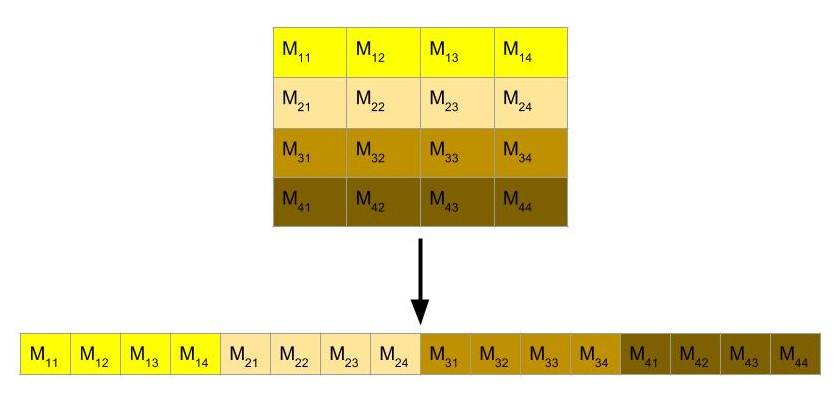
\includegraphics[width=\linewidth,height=12cm,keepaspectratio]{Figures/flatten}
		\caption[flattening 2d matrix]
		{flattening 2d matrix to row-wise 1d vector}
	
	\end{figure}
			
	The embedding process could be easily generalized if c is vectorized to values - set, then the dimension of $\alpha$ would be:\\ 
	$\prod_{i=1}^{2n}c_i$ , which equivalent to the number of vertices in the “discretized” space of the problem.
	In order to finally receive a distance/similarity/dis-similarity function, we apply inner product between $\alpha$  vector and a learned weights vector (equivalent to the $W$ matrix from the $1D$ scenario).
	
	
	
	\begin{algorithm}
				\caption{Embedding Method for ID N-Dimensional Pairs dataset}
				\begin{algorithmic}
				 
				
				\REQUIRE $L$ sized, vectorized n-dimensional pairs dataset
				\REQUIRE set of centers per dimension - $C$
				\ENSURE $\overrightarrow{\phi}$: $L$ sized set, embedded, sparse vectors\\
				
				\STATE \textbf{Find centers vectors}
				\STATE V shall be a set of centers - vectors
				\FORALL{dim in $n$}  
				\STATE $V_{dim} \leftarrow centers \quad vector \quad per \quad dim$
				\ENDFOR
				
				\STATE \textbf{Find embedded coefficients for all dataset}
				\STATE $\overrightarrow{\phi} = C^{2n}$ length empty $\overrightarrow{\phi}$ embedded vectors
				\STATE concat all pairs into a single vector $\overrightarrow{p}$
				\FORALL{$\overrightarrow{p}$ in $L$}
				\STATE find $\overrightarrow{p}$ bounding hypercube 
				\STATE find $\overrightarrow{p}$ bounding simplex (permutation method)
				\STATE $\overrightarrow{\lambda} \leftarrow$ find $\overrightarrow{p}$ barycentric coefficients 
				\STATE $\overrightarrow{\hat{\lambda}} \leftarrow$ normalize($\overrightarrow{\lambda}$)
				\ENDFOR
				\STATE \textbf{Assign}
				\FORALL{$\overrightarrow{\phi}$ in $emb-set$}
				\STATE $inds \leftarrow$ find vertices from hypercube and simplex locations
				\FORALL{$i$ in $inds$}
				\STATE $\overrightarrow{\phi}_{(i)} \leftarrow \overrightarrow{\hat{\lambda}}(j(i))$ -- j is the assigning function between the coef. vector and embedding vector
				\ENDFOR
				\ENDFOR
				
				\RETURN $\overrightarrow{\phi}$
	
				
				\end{algorithmic}
			\end{algorithm}
	
	
\section{Non-euclidean non-embeddable Metrics example}

Let us display an example of a useful application to IDDND method.
As described in the introduction chapter{}, IDDND method overcomes two main issues:

\begin{enumerate}
	\item \textbf{distortion} issues cause when applying euclidean metrics on a given arbitrary dataset. 
	\item \textbf{Metrics} are not necessarily applied on dissimilarities problems
\end{enumerate}

We demonstrate a theoretical use case constrained by those 2 conditions, and see how our method would overcome those and fits a proper model to a non-embeddable dataset.
\\ \\ 
\newcommand{\centert}{2.66}

\begin{figure}[h]
	\centering

	\begin{tikzpicture}

	\draw (0,0) node[anchor=north]{$\overrightarrow{x_2}$}
	-- (8,0) node[anchor=north]{$\overrightarrow{x_3}$}
	-- (4,6.928) node[anchor=south]{$\overrightarrow{x_1}$}
	-- cycle;
	
	%\draw (4,\centert) node[anchor=north]{$\overrightarrow{x_0}$}
	\draw (0,0) -- (4,\centert);
	\draw (8,0) -- (4,\centert);
	\draw (4,6.928) -- (4,\centert);
	\node at (4.5,2.9) {$\overrightarrow{x_0}$};
	
	\node[green] at (1.8,3.7) {$2$};
	\node[green] at (6.2,3.7) {$2$};
	\node[green] at (4,-0.5) {$2$};
	
	\node[green] at (3.8,4.7) {$1$};
	\node[green] at (2.2,1.8) {$1$};
	\node[green] at (5.8,1.8) {$1$};
	
	\draw[black,fill=black] (0,0) circle (.5ex);
	\draw[black,fill=black] (8,0) circle (.5ex);
	\draw[black,fill=black] (4,6.928) circle (.5ex);
	\draw[black,fill=black] (4,\centert) circle (.5ex);
	
	\end{tikzpicture}
	
	\caption[triangle non-embeddable dataset]
	{this is a scheme of a non-embeddable dataset}
	
	\end{figure}
	
	This theoretical set form applies a non-euclidean embeddable metrics, which we now prove that a euclidean metrics is unable to embed it.
	Based on euclidean metrics assumptions, assumed there is an integer $k$ , such that a function $f$ applies:
	
	\begin{equation}
	f \: : \: \{  \overrightarrow{x_1}, \overrightarrow{x_2} , \overrightarrow{x_3} , \overrightarrow{x_4}\} \rightarrow \Re^k
	\end{equation}
	
	Where $\overrightarrow{x_i}$ are samples from each one of data centers, and $f$ preserves the distances. \\ \\
	
    As triangle-inequality is tight for: $\overrightarrow{x_4} , \overrightarrow{x_1} , \overrightarrow{x_2}$ ,\\ \\
	
	$f(\overrightarrow{x_4}) ,f(\overrightarrow{x_1}) ,f(\overrightarrow{x_2})$ are collinear in $\Re^k$
	
	From set formation symmetry property, the same colinearity applies on:
	
	$f(\overrightarrow{x_3}) ,f(\overrightarrow{x_1}) ,f(\overrightarrow{x_2})$
	
	This common colinearity of those tuples leads to the following equation:
	
	$\left \| f(\overrightarrow{x_4}) - f(\overrightarrow{x_3})  \right \|_2 == 0$
	
	But this fact is contradicting that 
	
	$ d(\overrightarrow{x_4}\ , \overrightarrow{x_3}) = 2 $
	
	
	





	




